\documentclass[letterpaper]{article}
\usepackage[submission]{aaai2027}
\usepackage[hyphens]{url}
\usepackage{graphicx}
\urlstyle{rm}
\def\UrlFont{\rm}
\Urlmuskip=0mu plus 1mu\relax
\makeatletter\def\UrlBigBreaks{\do\/\do\.}\makeatother
\usepackage{natbib}
\usepackage{caption}
\frenchspacing
\usepackage{booktabs}
\usepackage{amssymb}
\usepackage{array}

\pdfinfo{
/TemplateVersion (2027.1)
}

\setcounter{secnumdepth}{0}

\title{CaliberGraph: Coverage-Caliber Witness Compilation for Multi-Business-Domain Governed Metrics}
\author{Anonymous Submission}
\affiliations{}

\begin{document}

\maketitle

\begin{abstract}
Industrial text-to-SQL systems increasingly succeed at finding relevant data, yet governed business intelligence requires more than plausible retrieval or executable SQL: an answer must jointly satisfy metric scope, hierarchy grain, physical coverage, time, and disclosure policy. Existing systems expose these rules as metadata or prompt context, but do not require a verifiable proof of their joint satisfaction.
We introduce \textsc{CaliberGraph}, a governance-semantic compiler that turns governance artifacts into executable constraints. Its central abstraction is a \emph{coverage-caliber witness}: a structured certificate that binds a candidate answer to all required metric, data, temporal, and policy conditions. CaliberGraph answers only when such a witness can be constructed; otherwise, it refuses with a typed failure certificate. We also introduce \textsc{MetricCaliberBench} to evaluate this governed-validity gap independently of candidate discovery.
Our evaluation shows that governance failures persist even with strong retrieval and prompting. Capable language models can emulate complete contracts, but compilation provides fast, model-independent, and auditable enforcement. The key insight is that governed finalization is best treated as constraint compilation rather than another retrieval or prompting problem.
\end{abstract}

\begin{links}
\link{Code and data}{https://anonymous.4open.science/r/calibergraph-artifact-70FA}
\end{links}

\section{Introduction}

Natural-language database interfaces have advanced rapidly through LLMs, text-to-SQL, schema linking, and retrieval augmentation \citep{spider,bird,spider2,autolink2026}. These systems increasingly recover the relevant tables, fields, and metrics; semantic layers (dbt, LookML, Cube) and safety-oriented NL2SQL (TrustSQL, SafeNLIDB) manage definitions, feasibility, and privacy---but none decides joint contract validity. Governed analytics thus poses a second question: \emph{is the requested answer valid under the business contract?}

A request such as ``complaint rate by category'' is correct only if metric identity, denominator scope, grain, filters, time binding, physical coverage, and answer/refuse policy are jointly satisfiable. A plausible SQL query can execute while dividing by the wrong population; a GraphRAG planner can retrieve both country and city while violating a finest-grain policy; and a safety-aware system can refuse sensitive data yet still answer an unsupported business metric---on a BIRD diagnostic only 0.078 of plausible SQL answers match all four governed readings (RQ2). We call the required proof object a \emph{coverage-caliber witness}. Figure~\ref{fig:arch}(a) grounds this gap on a released desensitized enterprise request.

The gap is not another candidate-retrieval problem: prompt-level GraphRAG exposes rules as text without requiring joint satisfaction, and a capable model can emulate a contract, but its behavior, context cost, and transport are model-dependent. Our insight is to treat governance metadata as a program---metric dependencies, hierarchy rules, coverage edges, valid-time anchors, and disclosure policies compile into typed constraints; a plan is admitted only if they construct a witness, otherwise the system returns a typed failure certificate and refuses (Figure~\ref{fig:arch}(b--d)).

We operationalize this insight with \textsc{MetricCaliberBench}. The protocol separates legal prediction inputs from scorer-only gold labels and organizes evidence by role: public-native (row-level behavior), enterprise-derived (real governance structure), controlled twins (mechanism isolation), and private or external assets (recurrence and scope). Three independent practitioners additionally reconstruct labels from released catalogs, so contract interpretability is measured rather than assumed.

We propose \textsc{CaliberGraph}, a governance-semantic compiler and constrained planner for NL2Metric. A linker proposes metric and dimension candidates, but a typed compiler decides whether the governance constraint families can construct a witness. The central empirical test is deliberately adversarial to our thesis: when candidate availability is saturated and competing validators see the same released rules, do failures remain without witness construction?

Our contributions are:
\begin{itemize}
    \item We introduce \textsc{MetricCaliberBench}, a reusable protocol for governed answerability with public/enterprise evidence groups, blind/gold separation, adjudication rules, circularity audits, and key-free scoring.
    \item We propose \textsc{CaliberGraph}, a coverage-caliber witness compiler that converts governance contracts into executable checks and typed missing-witness certificates.
    \item We establish the accuracy--cost--guarantee boundary with real MetricFlow, full-contract prompting, validator-feedback replanning, paired tests, ablations, and human validity, including a disclosed private-contract inversion (0.981 vs.\ 0.925). Accuracy parity is the predicted outcome: strong prompting can emulate a contract at $\sim$115k tokens per online call, while compilation enforces the same conformance model-independently at zero online finalization calls (linking shared) with a typed certificate.
\end{itemize}

None of this is an accuracy leaderboard: conformance to our own contract is a reference point; discriminating comparisons occur only on runnable controls and non-saturated or external contracts.

\section{Task: NL2Metric-Caliber}

\paragraph{Problem setting.}
Let $q$ be a natural-language analytics request and $G=(V,E)$ a typed governance graph containing metric, dimension, physical-field, coverage, policy, and alias nodes. The system outputs $y=(a,m,\Delta,t,\tau)$, where $a\in\{\textsc{answer},\textsc{refuse}\}$, $m$ is a governed metric identifier or empty, $\Delta$ is a governed dimension set, $t$ is a time binding, and $\tau$ records decision evidence.

\paragraph{Coverage-caliber witness.}
An answerable plan must admit
\[
w=(m,\Delta,t,T,\Phi,\Pi,\mathcal{A},\mathcal{S}),
\]
where $T$ is an authorized physical table or public source, $\Phi$ maps logical dependencies to physical fields, $\Pi$ records active policies, $\mathcal{A}$ records valid-time/as-of binding, and $\mathcal{S}$ records disclosure constraints. A valid witness jointly satisfies metric identity, numerator/denominator scope, grain, field and table coverage, time, and policy compatibility. If any required element is absent, the system must refuse rather than silently drop the constraint.

\paragraph{Correctness.}
We score metric identity, exact governed dimension grain, their joint correctness, and answer/refuse precision and recall. An executable query is not necessarily correct: execution does not detect a wrong denominator, invalid hierarchy level, or prohibited disclosure. Time and trace audits are mapped in the supplement rather than folded into an opaque aggregate score.

\paragraph{Contract validity.}
Gold labels define a versioned governance contract, not a universal language distribution. Three BI/governance practitioners, uninvolved in authoring the labels or CaliberGraph, independently annotate a stratified 120-case sample from the 898 released base cases (13.4\%). Action agreement is Fleiss $\kappa{=}0.968$; majority vote matches released gold on 117/120 actions, 93/93 metric ids and 92/93 dimension sets given answer. Replacing \emph{all} four majority--gold disagreements (three ICT actions and one Chinook grain) changes CaliberGraph from 1.000 to 0.981/0.975 on those layers but preserves every method ranking. Anonymized sheets and the deterministic recomputation are released. This validates contract interpretability, not unobserved physical bindings. Exact scores therefore denote fixed-contract conformance; the falsifiable empirical claim concerns the reliability and cost of implementing that contract after candidates are available.

\section{CaliberGraph}

CaliberGraph separates \emph{relevance} from \emph{validity}: candidate linking proposes plausible metrics and dimensions; compilation turns governance metadata into an executable constraint system $\Gamma(G)$; witness-guided finalization returns a satisfying assignment or a typed failure certificate. Figure~\ref{fig:arch} walks a released enterprise request through the contract gap (a), one-time compilation (b), conjunctive certification (c), and the answer/refuse decision (d); \textbf{M1}--\textbf{M3} are exactly the modules ablated in RQ3. Card and certificate fields follow released traces verbatim: $q'$ is a released one-factor plan mutation (dimension set changed to Product Color; a controlled mutation, not a verbatim production request) whose partial witness records $T.\mathrm{status}{=}\mathrm{missing}$; gray witness slots originate from the candidate and pass validation, blue slots are contract-bound.

\begin{figure*}[t]
\centering
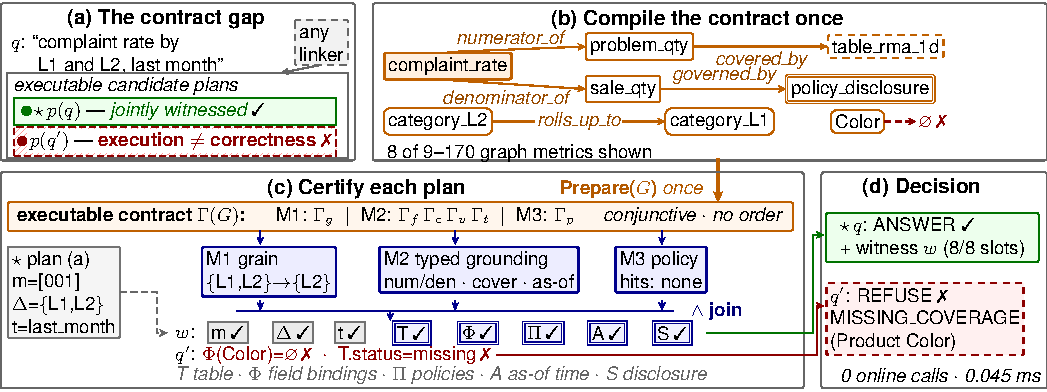
\includegraphics[width=\textwidth]{figures/fig1_calibergraph.pdf}
\caption{Retrieval proposes; compilation proves: the linker's candidate (a) is certified against the compiled contract (b) by M1--M3 (c); $q$ answers with a witness, $q'$ ($\Delta\!\to$Color) refuses with a typed certificate (d)---finalization: 0 online calls, 0.045\,ms.}
\label{fig:arch}
\end{figure*}

\subsection{Typed Governance Graph}

Metric nodes store formulas, dependencies, numerator/denominator roles, default time, allowed dimensions, and disclosure attributes. Dimension nodes store aliases, hierarchy, and grain. Physical-field and coverage nodes connect logical requirements to authorized assets. Policy nodes encode comparison, refusal, disclosure, and time behavior. Edges include \texttt{alias\_of}, \texttt{requires\_field}, \texttt{rolls\_up\_to}, \texttt{covered\_by}, and \texttt{governed\_by}; Figure~\ref{fig:arch}(b) draws a released fragment of $G$, with border styles encoding node types.

\subsection{Coverage-Caliber Compilation}

CaliberGraph compiles six constraint families: field contracts; metric-caliber dependencies; hierarchy grain; physical coverage; temporal/disclosure requirements; and answer/refuse policy. Retrieved graph text can describe these rules, whereas $\Gamma(G)$ must execute them jointly. A failure identifies the missing witness type: metric identity, denominator/scope, hierarchy grain, physical coverage, temporal binding, disclosure, or answerability.

For a request $q$ and candidate plan $p=(m,\Delta,t,T)$, compilation yields
\[
\Gamma(q,p,G)=\Gamma_f\land\Gamma_c\land\Gamma_g\land
\Gamma_v\land\Gamma_t\land\Gamma_p,
\]
where the subscripts denote field, caliber, grain, coverage, temporal/disclosure, and policy constraints. An answer is admitted iff there exists a binding $w$ such that $w\models\Gamma(q,p,G)$. This conjunction matters: a metric may be individually valid while its denominator is unavailable under a requested filter, or a table may contain every named field while its disclosure tier forbids the requested output.

\paragraph{Compiled checks (M1--M3).}
The six families execute inside three online modules, named consistently in Figure~\ref{fig:arch}(c), the planning pseudo-code (supplement), and the RQ3 ablation. \textbf{M1 (grain compiler, $\Gamma_g$)} projects requested dimensions onto allowed hierarchy paths and applies the configured grain rule. \textbf{M2 (typed grounding, $\Gamma_f\land\Gamma_c\land\Gamma_v\land\Gamma_t$)}: $\Gamma_f$ normalizes aliases and checks display/filter roles; $\Gamma_c$ expands formulas into required numerator, denominator, and scoped dependencies; $\Gamma_v$ binds every logical dependency to an authorized physical field and table at compatible grain; $\Gamma_t$ checks event time, valid time, as-of anchors, and release tier. \textbf{M3 (policy compiler, $\Gamma_p$)} applies comparison, unsupported-metric, SQL/DDL, sensitivity, and disclosure rules in a fixed priority order. The modules are conjunctive constraint groups; pseudo-code line order is an implementation detail, not a pipeline.

The released implementation executes these checks rather than emitting a template trace; parsing, hierarchy resolution, and per-layer binding mechanics are in the supplement. A check unavailable in a released contract is marked \emph{inactive} rather than silently passed (coverage is active for 32/32 Iowa and 426/510 MultiGov cases; the rest expose no required public binding), and every prediction records active status, evidence, missing bindings, and any refusal certificate.

\subsection{Witness-Guided Planning}


The grain compiler collapses each requested hierarchy path to the governed finest grain; the coverage compiler verifies dependencies, filters, table grain, time, and authorization. No online LLM call is used after governance artifacts are built; with $k$ candidates, checking is $O(k(d_m+r_m))$ for a candidate's governed dimensions $d_m$ and active requirements $r_m$.

\paragraph{Contract-relative soundness and certificates.}
\looseness=-1 \textbf{Proposition 1 (contract-relative soundness).} \emph{If finalization emits \textsc{answer} with witness $w$, then $w$ satisfies every active family of $\Gamma(G)$; no emitted answer violates the compiled public contract.} Proof sketch: every \textsc{answer} path of the planner (pseudo-code in the supplement) returns only after all active families hold; otherwise the implementation records the first unsatisfied family and all missing dependencies as a typed certificate. The guarantee is one-sided and contract-relative: refusing everything is vacuously sound, so it must be read with refusal precision 1.000 (by construction) and empirical recall 0.778 (private contract); soundness is relative to the released contract, not an unobserved universal one. A seven-case counterfactual suite mutates field identity, ratio dependencies, grain, coverage, time, and policy authorization one at a time; a five-case MultiGov suite removes only the current metric's numerator, denominator, or physical binding while retaining other metrics' same-domain edges. All twelve expected outcomes are recovered, distinguishing metric-specific checking from a constant trace or a domain-level shortcut.

\section{Experimental Design}

We organize experiments by claims. Five research questions determine the order and role of every comparison:
\begin{itemize}
    \item \textbf{RQ1---Overall effectiveness:} Does the complete method outperform retrieval, prompt, execution, and validation baselines?
    \item \textbf{RQ2---Post-linking bottleneck:} Do errors remain when intended candidates and released semantic rules are already available?
    \item \textbf{RQ3---Module contribution:} Which compiled components produce the gain?
    \item \textbf{RQ4---Robustness and external validity:} Does the conclusion survive wording, policy, model, and source changes?
    \item \textbf{RQ5---Efficiency and auditability:} What finalization cost is added, and can each decision be mechanically inspected?
\end{itemize}

\subsection{Evidence Groups}

Four groups separate externally public data from enterprise-derived evidence: \emph{public-native} (Iowa 32; Chinook 40; BIRD 206 diagnostics), \emph{enterprise-derived public} (MultiGov 510; IndustrialCaseText (ICT) 157), \emph{controlled public stress} (GovTwin 159 base, 468 perturbations, 159 paraphrases), and \emph{supporting} evidence (DataHub inventory; external anchors). The 1525 public scored cases exclude the BIRD diagnostics; the full group/role table, schemas, construction procedures, privacy boundaries, and per-dataset statistics are in the supplement.

IowaLiquor releases public rows, a semantic layer, and executable SQL; MultiGov releases anonymized governance structure from 12 production versions; IndustrialCaseText releases desensitized requests with separated blind/gold files; GovTwin is a controlled semantic twin. Private assets establish recurrence only---no private aggregate is headline supporting evidence; the disclosed inversion is a boundary result. Per-dataset construction details are in the supplement.

\subsection{Comparison Baselines}

Baseline selection follows the alternative explanation each family controls. \emph{Retrieval controls} (Direct Keyword and Schema-RAG proxy) test whether catalog access alone is sufficient. \emph{Prompt planners} (LLM Direct, Schema-RAG, and GraphRAG) test compact context and graph neighbors; a separate full-contract prompting control (instructed execution) places the entire contract in one prompt. \emph{Execution controls} include an open SQLite planner and a real MetricFlow 0.211.0 engine. \emph{Validation controls} include semantic-layer and SQL post-hoc checks. The strongest runnable mechanism control iterates Schema-RAG planning with gold-free violations emitted by the same released typed checks for at most three repairs; it is deliberately a shared-validator control, not an independent semantic engine. \emph{Published-mechanism adaptations} use AutoLink-derived E3 candidate linking and SafeNLIDB-derived E3 guarding under the same NL2Metric interface (evidence level E3: a published mechanism on our interface, not upstream retraining); the E3 linking stage shares the unified backbone with the Schema proxy, so coinciding Iowa/MultiGov row values are same-origin by construction, not independent reimplementations. Oracle-candidate rows receive scorer metric identity by definition and remain diagnostics; our central conclusion rests on the complete runnable controls.

The family/capability matrix is in the supplement. The primary LLM comparison uses \texttt{deepseek-3.2}; a fixed 12-model enterprise-text panel tests model sensitivity, and the full-contract control adds \texttt{gpt-5.5} and \texttt{claude-opus-4-6} after transport canaries. Missing/API/parse failures are never imputed. The feedback protocol was frozen on 391 cases (Iowa-32, GovTwin-159, seeded MultiGov-200); the IndustrialCaseText-157 and full MultiGov-510 runs are labeled extensions, never called preregistered. Spider2-DBT, TrustSQL raw, DataBench, and LightRAG remain adjacent scope checks; MetricFlow is a real executed baseline sharing the released semantic project.

\subsection{Ablations and Metrics}

Overall comparisons use complete systems; module experiments remove one CaliberGraph capability (M1 grain compiler, M2 typed grounding, or M3 policy compiler). Metric accuracy checks governed metric identity; dimension accuracy requires exact governed grain; joint accuracy requires both; refusal precision/recall measure answerability behavior. We additionally report action-aware full-case correctness, paired exact McNemar tests, and deterministic cluster-bootstrap intervals; clustering uses metric groups for MultiGov and normalized-query groups for IndustrialCaseText.

\section{Results}

\subsection{RQ1: Overall Effectiveness}

\looseness=-1 Table~\ref{tab:overall} gives the central comparison before module analysis; its exact 1.000 rows are conformance references (Introduction). Full-contract prompting beats compact retrieval on Iowa and MultiGov but is inconsistent across layers. The shared-validator iterative control is substantially harder: it ties CaliberGraph on Iowa and reaches 0.971 on MultiGov-510 and 0.879 on IndustrialCaseText, residual differences of 0.029 and 0.121. Because the repair loop consumes our typed violations, these gaps compare execution procedures under shared checks, not independent semantic definitions; sharing our validator by design also bounds what shared rules can fix. Real MetricFlow \citep{metricflow2026} and the open SQL planner reach 0.625 and 0.562 joint on Iowa, respectively, showing that executable semantic queries are not by themselves governed witnesses. A deterministic alias-matching control (RapidFuzz, no witness) resolves metric identity on answerable MultiGov cases (1.000) yet scores 0.000 joint: zero-match fallback catches identity refusals, but every grain, coverage, and policy decision passes unchecked, so alias resolution is not caliber verification. An uncertainty-abstention control ($k{=}5$ consistency entropy, thresholds pre-registered) closes the last alternative route: all 37 would-be errors fall in the grain family and 7 of them (18.9\%) are zero-entropy confident mistakes, while the denominator-caliber stratum records zero errors on its 11 unanimously-sampled cases (entropy exactly 0.000; reported as underpowered). Metric-caliber errors are confident errors, invisible to abstention at any threshold (Figure~\ref{fig:dynamics}(c), axis truncated at 62\%; GovTwin's selective risk floors at .064; MultiGov attains zero risk only at 70.5\% coverage; strictest pooled point: 0.972 answered-joint, 30.1\% abstention, $5\times$ cost).

\begin{table}[t]
\centering
\small
\setlength{\tabcolsep}{2.5pt}
\begin{tabular}{lccc}
\toprule
Method & Iowa & MultiGov & ICT \\
\midrule
Keyword & .156/.000 & .000/.000 & .522/.250 \\
Schema proxy & .562/.000 & .320/.000 & .866/.250 \\
Open SQL e2e & .562/.000 & -- & -- \\
MetricFlow 0.211 & .625/.286 & -- & -- \\
AutoLink E3 & .562/.000 & .320/.000 & -- \\
SafeNLIDB E3 & .781/1.00 & .680/1.00 & .904/1.00 \\
Full-contract DS-3.2 & .875/1.00 & .855/1.00 & .822/.875 \\
Shared-val.\ repair & 1.00/1.00 & .971/1.00 & .879/1.00 \\
CaliberGraph (ref.) & \textbf{1.00/1.00} & \textbf{1.00/1.00} & \textbf{1.00/1.00} \\
\bottomrule
\end{tabular}
\caption{Overall comparison. Each cell is joint metric+dimension accuracy / refusal recall (higher is better for both). Full-contract and repair rows are full runnable controls; E3 denotes the released unified-backbone protocol. MultiGov is the full-510 layer (seeded-200 gives .865, used in RQ4--RQ5). ``--'' is non-applicable. Only the contract-conformance reference row is bolded; ties against it (e.g., repair on Iowa) are stated in the text rather than ranked.}
\label{tab:overall}
\end{table}

Against the strongest runnable control (not the easiest baseline), the action-aware full-case difference is .000 on Iowa (a tie), .029 on MultiGov (95\% cluster-bootstrap CI [.016,.045], exact McNemar $p{=}6.1{\times}10^{-5}$), and .121 on IndustrialCaseText (CI [.070,.181], $p{=}3.8{\times}10^{-6}$); intervals: 10{,}000 cluster replicates.

\subsection{RQ2: The Post-Linking Bottleneck}

Table~\ref{tab:mechanism} controls progressively stronger alternative explanations. Among answerable cases, E3 candidate availability is already 1.000 on Iowa and MultiGov and 0.973 on IndustrialCaseText (four metric-candidate misses; supplement); Figure~\ref{fig:dynamics}(a) sweeps the retrieval budget: metric recall climbs from 145/149 ($k{=}1$) to 149/149 ($k{\ge}3$), yet 22--31 final errors persist (28--31 once recall saturates). Supplying the entire contract in one prompt still yields 0.875, 0.855, and 0.822. Shared typed-validator feedback repairs every detectable violation and lifts the three layers to 1.000, 0.971, and 0.879, respectively. It nevertheless leaves 15 MultiGov and 19 IndustrialCaseText candidate-selection errors that pass all exposed checks but choose the wrong metric or dimension set. These are not direct failures of an active witness constraint: iterative feedback repairs only the violations its validator can name. Figure~\ref{fig:dynamics}(b) traces this: one round repairs nearly every nameable violation; GovTwin, seeded MultiGov-200, and IndustrialCaseText then plateau at residual errors of .019, .045, and .121 (full-510 extension: .029), the validator-invisible floor, and only Iowa closes (bars in Figure~\ref{fig:dynamics}(b): final-round Wilson 95\% CIs). The remaining accuracy delta therefore combines deterministic candidate binding with compiled validation; we do not attribute it to witness checking alone.

\begin{figure*}[t]
\centering
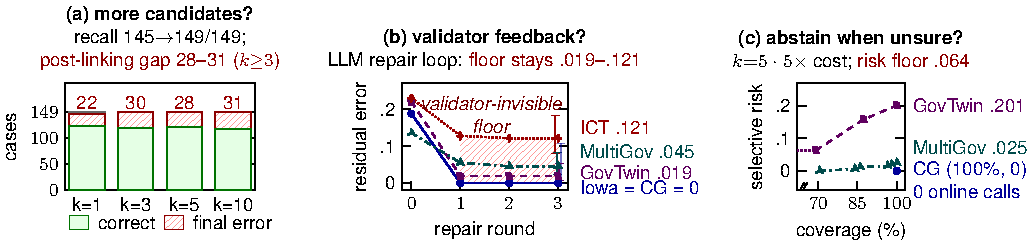
\includegraphics[width=\textwidth]{figures/fig2_floors.pdf}
\caption{Three online-LLM escape routes leave a residual floor (Iowa closes); compilation removes it: more candidates (a), validator feedback (b), abstention (c); zero-call CaliberGraph (CG) reaches $(100\%,0)$. Wilson 95\% CIs; (c) truncated at 62\%.}
\label{fig:dynamics}
\end{figure*}

\begin{table}[t]
\centering
\small
\setlength{\tabcolsep}{2pt}
\begin{tabular}{lcccc}
\toprule
Evidence & Candidate & Full-ctr. & Repair & CaliberGraph \\
\midrule
Iowa SQL & 1.000 & .875 & 1.000 & 1.000 \\
MultiGov & 1.000 & .855 & .971 & 1.000 \\
IndustrialCaseText & .973 & .822 & .879 & 1.000 \\
\bottomrule
\end{tabular}
\caption{Post-linking controls. Candidate availability is measured on answerable cases; other columns are all-case joint accuracy. MultiGov is the full-510 layer (seeded-200: .865). Repair receives only gold-free typed violations and at most three retries.}
\label{tab:mechanism}
\end{table}

Physical coverage is not silently credited when the contract lacks a binding: 458 of the 699 headline cases activate coverage (32 Iowa, 426 MultiGov), 241 do not (84 MultiGov, 157 ICT). On the active stratum, full-contract prompting, repair, and CaliberGraph score 0.867, 0.974, and 1.000 (0.813, 0.909, and 1.000 on the inactive stratum, which evaluates metric/grain/policy conformance only).

The released certificates make the missing operation concrete. An Iowa query for sales by county and city executes while grouping by both, but the contract requires city grain. An IndustrialCaseText request containing two segment levels is finalized with both levels instead of the governed finer level. A MultiGov raw-identifier request retrieves a nearby metric but lacks a disclosure witness and must be refused. These are not candidate misses.

Public BIRD outputs provide an external SQL diagnostic rather than a governed leaderboard: GPT-4-Turbo recovers tables at 0.830 and dimensions at 0.903, yet only 0.078 simultaneously match operator, measure, table, and grouping.

\subsection{RQ3: Module Contributions}

Table~\ref{tab:ablation} separates whole-system comparison from component evidence, ablating exactly the three modules of Figure~\ref{fig:arch}. Removing M1 (grain compiler) reproduces the dominant hierarchy failure and reduces GovTwin joint accuracy from 1.000 to 0.736. Removing M2 (typed grounding---the graph-constraint checks) further reduces joint accuracy to 0.679 and eliminates refusal behavior; removing M3 (policy compiler) leaves metric/grain planning largely intact but sets refusal precision and recall to zero. The M1 effect transfers to public sources: joint accuracy drops from 1.000 to 0.525 on Chinook \citep{chinook} and from 1.000 to 0.680 on MultiGov.

\begin{table}[t]
\centering
\small
\setlength{\tabcolsep}{3pt}
\begin{tabular}{lccc}
\toprule
GovTwin variant & Metric & Dim. & Joint/Ref.P/R \\
\midrule
Full CaliberGraph & 1.000 & 1.000 & 1.000/1/1 \\
$-$ M1 grain compiler & 1.000 & .736 & .736/1/1 \\
$-$ M2 typed grounding & .943 & .736 & .679/0/0 \\
$-$ M3 policy compiler & .943 & 1.000 & .943/0/0 \\
\bottomrule
\end{tabular}
\caption{Component ablation on 159 GovTwin base cases; M1--M3 are the modules of Figure~\ref{fig:arch}.}
\label{tab:ablation}
\end{table}

Query families explain the deltas: on MultiGov, AutoLink- and SafeNLIDB-derived controls both score 0.000 on finest-grain traps; the safety guard lifts policy-refusal accuracy 0.000$\to$1.000, but only CaliberGraph reaches 1.000 on both families: linking, refusal guarding, and witness compilation solve different stages.

\subsection{RQ4: Robustness and External Validity}

\paragraph{Wording and policy robustness.}
CaliberGraph reaches 1.000 on 159 frozen paraphrases, 0.987 on 468 deterministic perturbations, and 1.000 on 114 deduplicated IndustrialCaseText groups; the strongest published-mechanism control (SafeNLIDB E3) scores 0.736/0.718/0.736 on the GovTwin variants and 0.904/0.868 on exact/deduplicated IndustrialCaseText. A lenient parent+child policy lifts E3 to 0.975, yet CaliberGraph remains best, not an exact-grain scoring artifact (full table in the supplement).

\paragraph{Model sensitivity.}
The fixed 12-model GraphRAG panel covers 60 stratified enterprise-text cases; a harder control reproduces the complete 375k-character released MultiGov contract in each prompt (end-of-prompt canaries pass). On the same seeded 200 cases, \texttt{deepseek-3.2}, \texttt{claude-opus-4-6}, and \texttt{gpt-5.5} reach 0.865, 0.985, and 1.000 joint accuracy. opus's three errors are over-refusals from reading \texttt{coverage\_required=false} as unavailable; gpt-5.5 has none. Prompt-failure magnitude is model-specific, and we do not claim an LLM cannot implement the contract. Emulation still requires one long online call per request and gives no by-construction certificate; compilation is model-independent after governance construction.

\looseness=-1 Pre-registered extensions bound this emulation ability. \emph{Breadth}: the same full-contract protocol on the four remaining public layers gives gpt-5.5 1.000 (Iowa-32), 0.994 (GovTwin-159), 0.925 (Chinook-40), but only 0.860 on the 157 real desensitized enterprise requests (protocol-literal; 0.882 completed-subset; opus 0.764; table in supplement). Emulation is near-perfect where contract and request text are clean and degrades where request language is noisy. The semantic residuals are over-refusals and near-synonym caliber confusions, the families CaliberGraph decides by construction. \emph{A private non-saturated contract} (159 enterprise cases): CaliberGraph scores 0.925; of its 12 errors, 3 are pre-registered \emph{policy divergences} (the released policy itself disagrees with the private gold, capping any policy-compliant system at 156/159), and the remaining 9 are within-policy binding errors. Instructed execution reaches 0.780 (deepseek) and 0.723 (opus), but 0.981 with gpt-5.5---significantly \emph{above} CaliberGraph (exact McNemar $p{=}0.0039$): it repairs the 9 within-policy errors, loses none, and stops at the 3 policy-divergence cases, matching the released-policy ceiling of 156/159 in all three pre-registered passes (157/159 per-case agreement; Table~\ref{tab:privatearms}). The frontier model is the more faithful executor of the released policy here, but the win is not free: about 115k prompt tokens and one online call per request (Table~\ref{tab:buys}, Figure~\ref{fig:pareto}).

\emph{An external-ecosystem contract} (pre-registered) addresses catalog-authorship circularity: a third-party semantic manifest by the MetricFlow upstream project (dbt Labs)---not written by us---is mechanically converted to a 119-metric contract and 122 template cases. CaliberGraph's exact conformance (1.000, every stratum) transfers by construction through the released converter. The discriminating evidence is model divergence under the same mechanical gold: full-contract gpt-5.5 reaches 1.000 (zero discordance) while deepseek-3.2 reaches 0.811 ($p{=}2.4{\times}10^{-7}$) with the same failure families as on our layers---a split authorship circularity cannot explain. All artifacts are released; a further pre-registered SecureSQL anchor bounds what is compilable at all (Limitations).

On the same private contract, validator-feedback replanning against the compiled policy converges all three families to 0.899--0.937, zero regressions (Table~\ref{tab:privatearms}). We claim no accuracy superiority over frontier prompting on this set (Table~\ref{tab:buys}); the inversion is fully disclosed and read as \emph{contract centrality}: the strongest model wins by executing the compiled contract, mid-tier models do not, and compilation alone delivers the same conformance model-independently at zero online finalization calls (linking shared), refusal precision 1.000 by construction relative to the released contract (recall 0.778 empirical).

\begin{table}[t]
\centering
\small
\begin{tabular}{lccc}
\toprule
Arm (private 159 cases) & Joint$\uparrow$ & Ref.\ P$\uparrow$ & Ref.\ R$\uparrow$ \\
\midrule
Instr-exec (DS-3.2) & .780 & .421 & \textbf{.889} \\
Instr-exec (opus-4-6) & .723 & .412 & .778 \\
Instr-exec (gpt-5.5) & \textbf{.981} & .875 & .778 \\
Replan (DS-3.2) & .899 & \textbf{1.000} & .778 \\
Replan (opus-4-6) & .937 & \textbf{1.000} & .778 \\
Replan (gpt-5.5) & .925 & \textbf{1.000} & .778 \\
CaliberGraph & .925 & \textbf{1.000} & .778 \\
\bottomrule
\end{tabular}
\caption{Frontier arms on the private non-saturated enterprise contract. Bold = column best (ties bolded). The gpt-5.5 instructed-execution accuracy equals the pre-registered released-policy ceiling (156/159). Anonymous per-case pairs are released; raw text is not.}
\label{tab:privatearms}
\end{table}

\paragraph{External anchors.}
Executed adjacent checks (69 Spider2-DBT third-party projects parsed; TrustSQL raw under its official evaluator; a fixed 145-question DataBench subset \citep{databench2024}; LightRAG \citep{lightrag2026} stopped at preflight) establish scope without being miscast as governed-answerability scores.

\subsection{RQ5: Efficiency and Auditability}

Table~\ref{tab:buys} condenses the dual-battlefield conclusion: emulation and compilation tie exactly where contract and request text are clean, diverge in opposite directions elsewhere, and differ categorically in cost and guarantees.

\begin{table}[t]
\centering
\small
\setlength{\tabcolsep}{2.5pt}
\begin{tabular}{lcc}
\toprule
 & Emulation & CaliberGraph \\
 & (gpt-5.5, full ctr.) & (compilation) \\
\midrule
MultiGov-200 (clean) & 1.000 & 1.000 \\
ICT-157 (noisy) & .860 & 1.000 (ref.) \\
Private (159) & \textbf{.981} & .925 \\
Prompt tokens/query & $\sim$115k & 0 \\
Latency/query & 7.24 s & 0.058 ms \\
Online LLM calls & 1 & 0 \\
Determ.\ replay & no & yes (17{,}160/17{,}160) \\
Refusal prec.\ (priv.) & .875 emp. & 1.000 by constr.\textsuperscript{$\dagger$} \\
Repair-loop oracle & --- & compiled policy \\
\bottomrule
\end{tabular}
\caption{What compilation buys. Accuracy rows are joint scores from RQ1/RQ4; CaliberGraph public rows are conformance references, the private row the disclosed inversion. Cost rows are finalization-stage; shared upstream linking cost is not claimed. \textsuperscript{$\dagger$}relative to the released contract; recall 0.778 empirical.}
\label{tab:buys}
\end{table}

\begin{figure}[t]
\centering
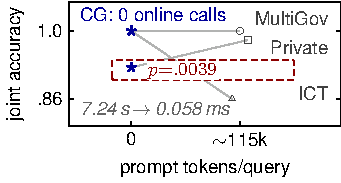
\includegraphics{figures/fig_pareto.pdf}
\caption{Emulation pays $\sim$115k tokens/query; zero-call compilation matches its public references ($p{=}.0039$).}
\label{fig:pareto}
\end{figure}

\looseness=-1 On the same MultiGov-200 full-contract condition (provider-reported input tokens), full-contract deepseek-3.2, opus, and gpt-5.5 spend 132{,}336, 141{,}016, and 115{,}363 prompt tokens per case at 38.05\,s, 9.10\,s, and 7.24\,s for 0.865, 0.985, and 1.000 joint accuracy. CaliberGraph finalization replays all 510 released decisions exactly over 20 repetitions at 0.058\,ms median (MultiGov-layer; pooled 0.045\,ms) with no online model call. This is a finalization-stage, not end-to-end linking, comparison, and supports no end-to-end speedup claim (Figure~\ref{fig:pareto}).

\looseness=-1 Auditability is exercised rather than asserted: all 858 predictions in the four base public contracts carry per-family records with unavailable checks marked inactive (Chinook in the supplement); the key-free rebuild regenerates splits, predictions, statistics, traces, and checksums.

\section{Related Work}

\paragraph{Text-to-SQL and schema linking.}
\looseness=-1 Spider and BIRD evaluate executable SQL \citep{spider,bird}; decomposition and multi-agent solvers push solving accuracy \citep{dinsql2023,macsql2023,chess2024}; Spider 2.0 adds enterprise workflows \citep{spider2}; AutoLink reframes industrial linking as iterative exploration \citep{autolink2026}. CaliberGraph addresses validity after candidates exist.

\paragraph{RAG and graph-based RAG.}
\looseness=-1 RAG and GraphRAG retrieve context, graph elements, or summaries \citep{rag,graphrag}; self-reflective retrieval adds a critique step \citep{selfrag}; ArchRAG and KG-alignment improve graph organization \citep{archrag2026,kgalignment2025}. CaliberGraph instead treats graph structure as executable constraints whose satisfying assignment is a witness.

\paragraph{Safe database interfaces and BI benchmarks.}
\looseness=-1 TrustSQL evaluates correct SQL for feasible requests and abstention otherwise \citep{trustsql2024}; SafeNLIDB targets privacy leakage \citep{safenlidb2026}; ambiguity-aware decoding \citep{ambiqt2023} resolves readings, not governed validity; BIS and BI-Bench move toward production BI evaluation \citep{bis2024,bibench2025}. MetricCaliberBench adds denominator-scope, grain, coverage, time, and disclosure contracts.

\paragraph{Semantic layers and governance.}
\looseness=-1 dbt Semantic Layer, LookML, and Cube define reusable metrics and access rules \citep{dbtsemantic,lookml,cube}; data-contract tools make fitness checks inspectable \citep{great_expectations_contracts}; semantic-layer-mediated agents guarantee compilability, not joint satisfiability \citep{smq2026}; time-travel covers as-of retrieval without a caliber witness \citep{temptabqa2023}. CaliberGraph compiles the same metadata into a joint witness procedure emitting a repaired plan or a typed refusal certificate.

\section{Limitations and Conclusion}

\looseness=-1 Iowa \citep{iowaliquor} uses public rows but authored labels; Chinook has 40 cases. MultiGov and GovTwin release anonymized governance artifacts, not rows; ICT releases desensitized requests and labels only. Coverage claims are contract-dependent (458/699 activate a binding; RQ2). Practitioner validation covers 120/898 cases; private physical mappings remain unvalidated. The external-ecosystem test removes catalog authorship, not pipeline authorship (pipeline components and gold derivation are ours; request text is templated). Cross-organization external validity is not established: the twelve MultiGov domains share one governance engine, and the dbt contract is the only externally-authored source. A pre-registered SecureSQL anchor bounds compilability: 19.9\% of its security conditions are non-mechanizable, and semantic-leakage leaves compilation (0.609, $n{=}932$) and frontier prompting (0.702, $n{=}300$) far below the human 94\% reference. Disclosure checks are by-construction only \emph{within structured contracts}. Exact McNemar assumes independent pairs; clustering makes case-level $p$-values anti-conservative. The private inversion rests on 9 discordant cases ($n{=}159$); anonymized per-case pairs are released. Caliber, grain, disclosure, refusal, and candidate-selection errors survive retrieval; MetricCaliberBench exposes them, and CaliberGraph decides them offline.

\bibliography{references}

\end{document}
